% !TEX root = ../thesis-example.tex
%
\section{Virtual projection parameters from real world camera}

To produce a virtual projection there are four unkowns to solve for:

\begin{my_list}
	\item Position of the real world camera
	\item Rotation of the real world camera
	\item Field of View (FoV) of the camera
	\item Distance between the HMD and the real world camera
\end{my_list}

Luckily the former two are solved by the tracking solution, thus can be used 
directly as transform for the virtual camera - ignoring an  additional offset 
from the actual controller to the camera, which is accounted for in the 
software.
\newline
The calculation of the corresponding distance between a 
camera and the Vive HMD to control the virtual projection parameters. Since 
both devices are tracked, one natively and the other with a controller as 
tracking position, it is calculated with the same euclidean distance as 
discussed earlier, with $C$ as camera position and $H$ as HMD position:

\eq{eq:zsort:distance}{
	Z = \sqrt{(C_X + H_X)^2 + (C_Y + H_Y)^2 + (C_Z + H_Z)^2}
}

\begin{figure}[htb]
	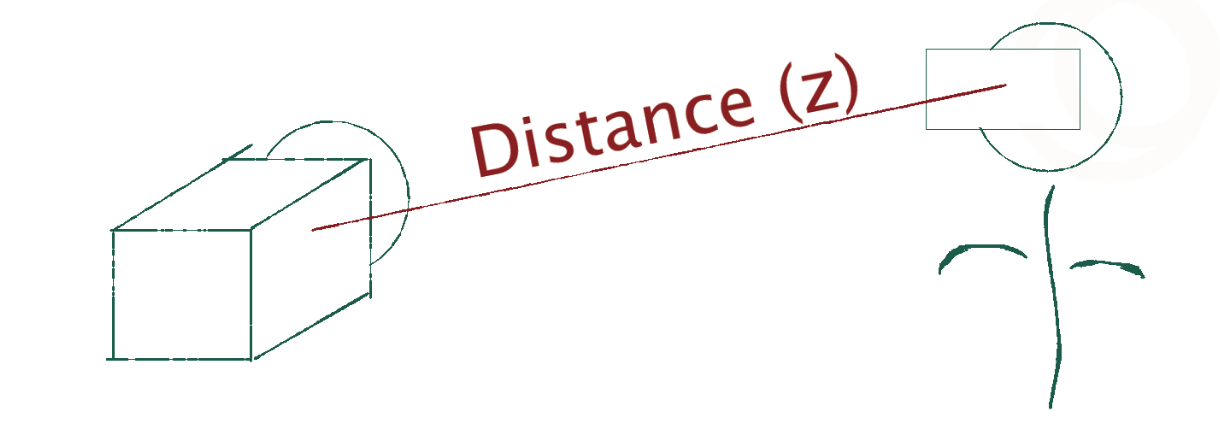
\includegraphics[width=\textwidth]{_raw_resources/composition/Composition-Z-Distance.png}
	\caption{Distance correlation}
	\label{fig:projection:distance}
\end{figure}

Another important projection parameter is the field of view. Most production 
cameras only declare a focal length on lenses - which makes sense in that 
context, since field of view is a constraint between sensor size and focal 
length. Through the specification sheet of the camera the current field of view 
can be calculated inside Unity, with the sensor height as $S_h$ and focal 
length as $F_l$, both in millimeter:

\eq{eq:zsort:fov}{
	FoV = 2*tan^{-1}\frac{S_h}{2 * F_l}
}

With that we have now all projection parameters for the virtual environment to 
generate an image that is at the same position as the real wolrd camera would 
look at.